\chapter{Аналитическая часть}

\section{Общие этапы нечёткого логического вывода}

На рисунке \ref{img:algo} представлена типовая структура нечёткой модели системы
с двумя входами и одним выходом.~\cite{book}

\begin{sidewaysfigure}
	\begin{center}
		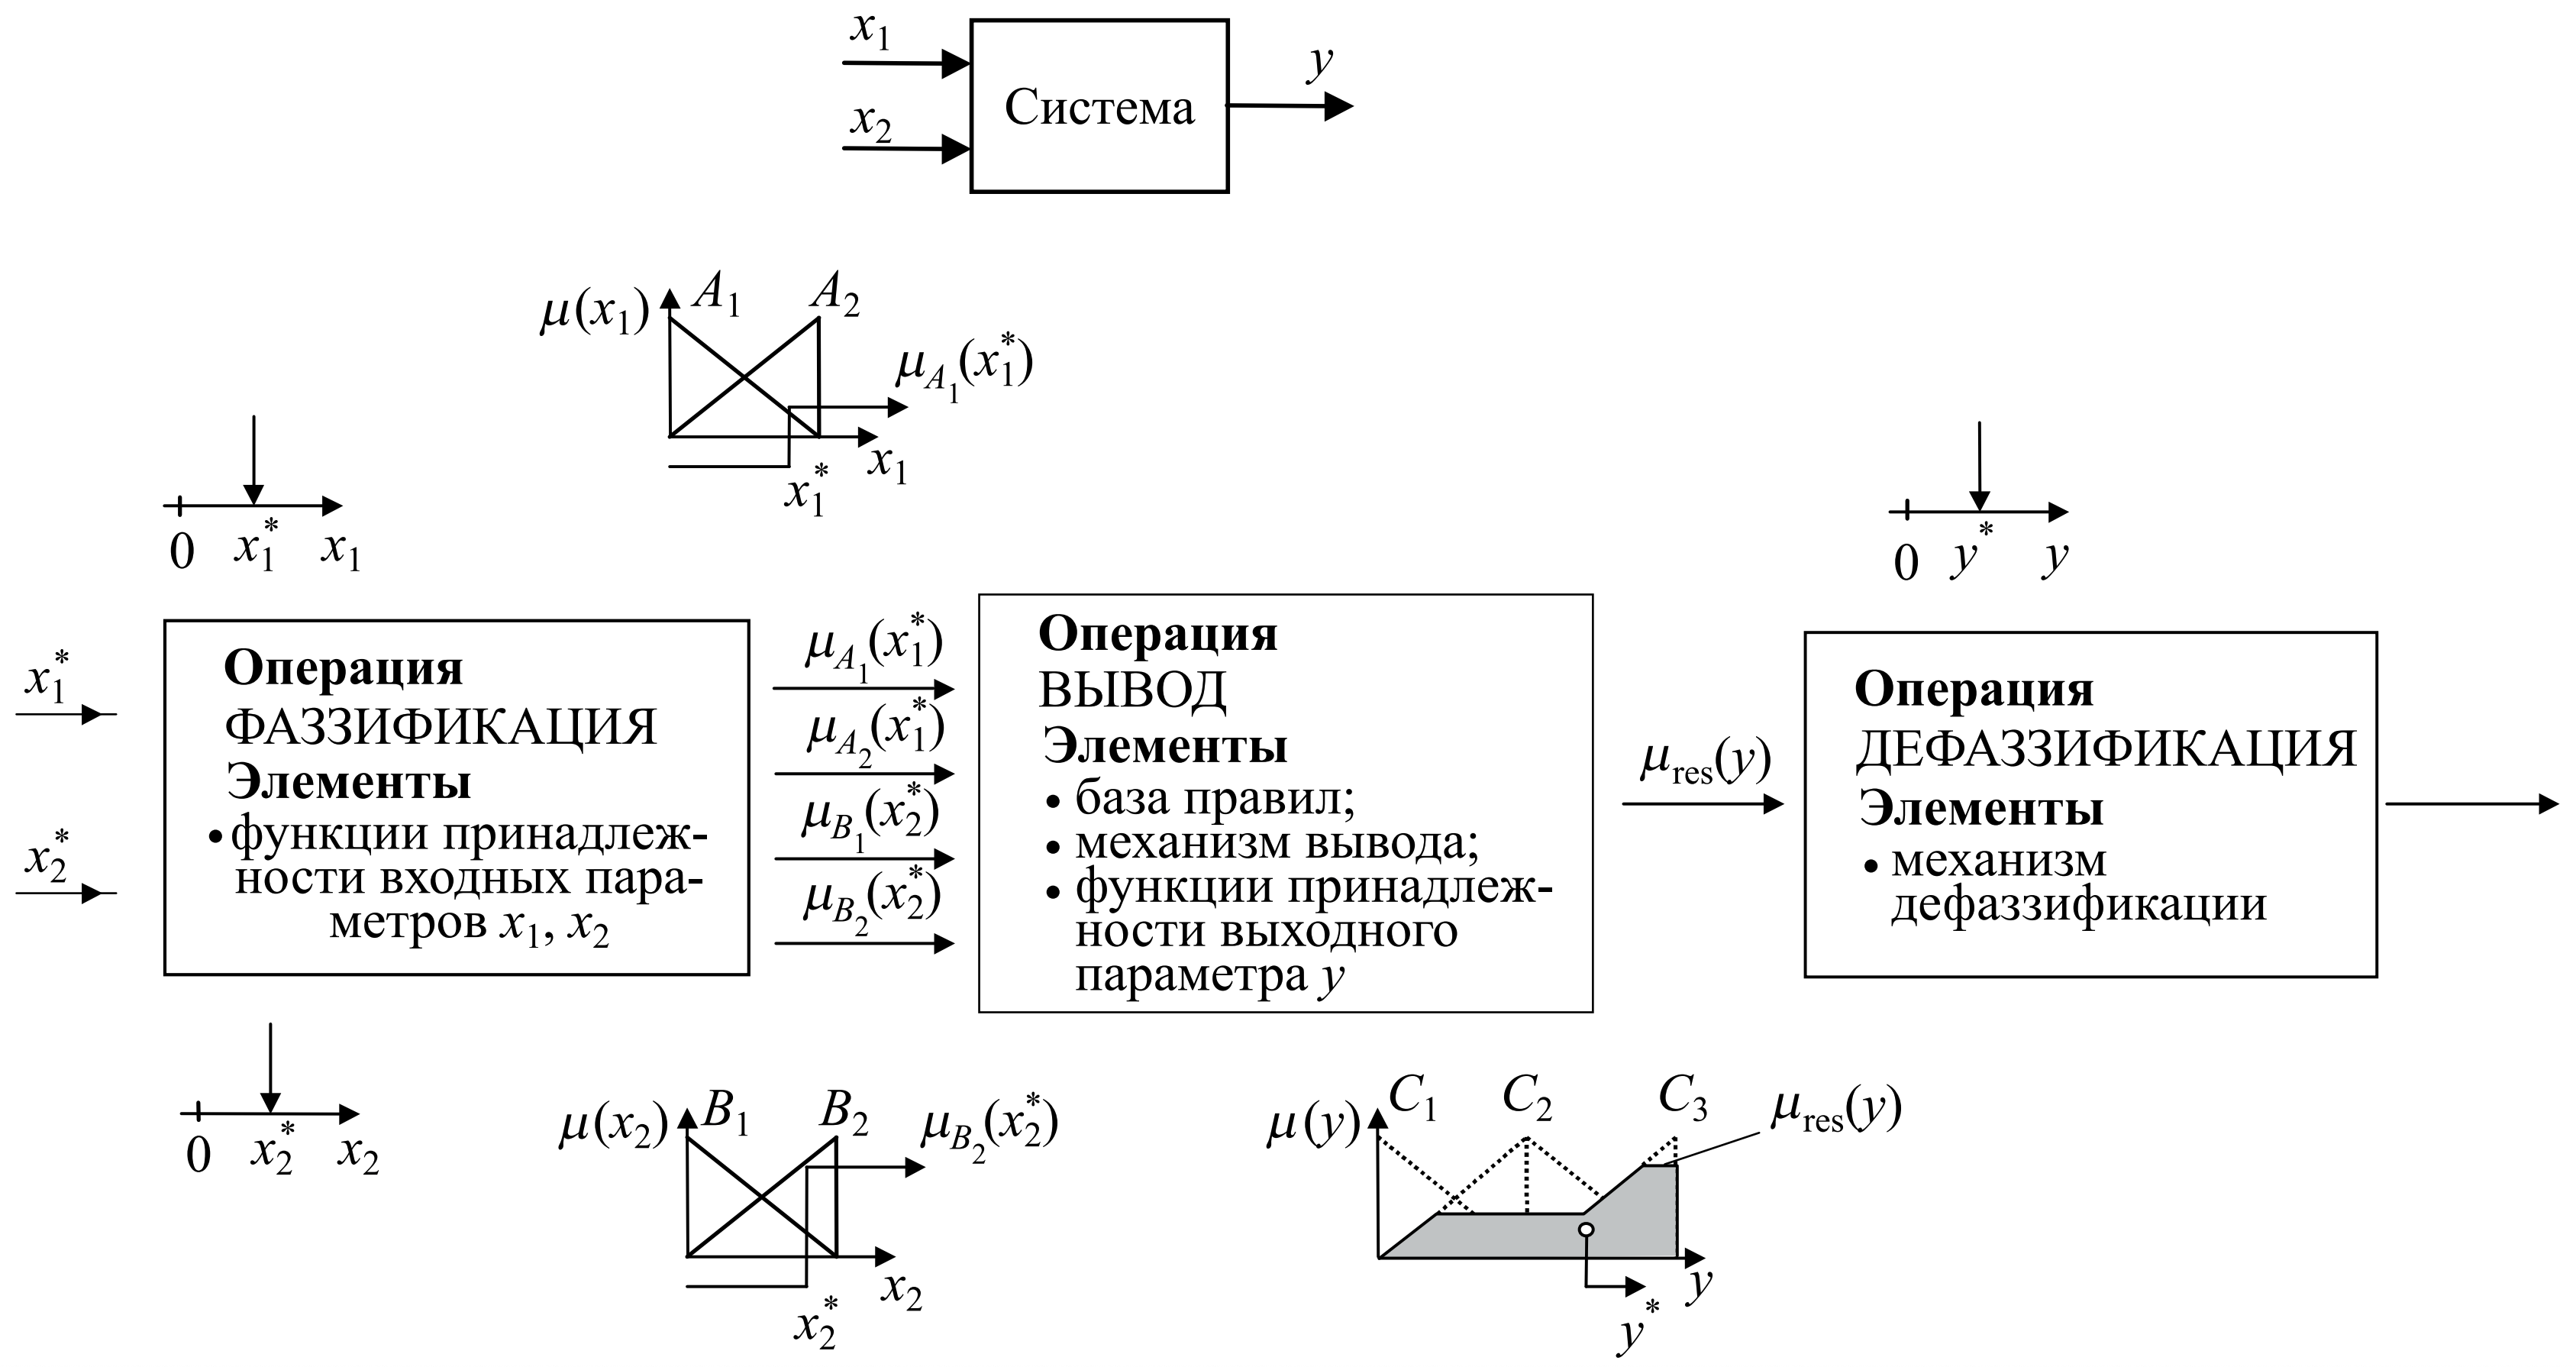
\includegraphics[width=0.9\textwidth]{images/algo.png}
	\end{center}
	\caption{Схема венгерского метода решения задачи о назначениях, часть 1}
	\label{img:algo}
\end{sidewaysfigure}

На входы нечёткой модели поданы два чётких числовых значения $x^*_1$, $x^*_2$. Блок «\textbf{ФАЗЗИФИКАЦИЯ}» \textbf{(FUZZIFICATION)} вычисляет их
степени принадлежности входным нечётким множествам $A_i$, $B_j$ . Для выполнения указанной операции блок фаззификации должен иметь доступ
к точно определённым функциям принадлежности $\mu_{A_i}(x1)$, $\mu_{B_j}(x2)$ входов.~\cite{book}

Вычисленные и представленные на выходе блока фаззификации степени принадлежности $\mu_{A_i}(x_1^*)$, $\mu_{B_j}(x_2^*)$ дают информацию о том, в какой
степени числовые значения $x^*_1$, $x^*_2$ принадлежат конкретным нечётким
множествам, т. е. насколько эти величины являются малыми (A1, B1)
или большими ($A_2$, $B_2$).~\cite{book}

Блок «\textbf{ВЫВОД}» \textbf{(INFERENCE)} на входе получает степени принадлежности $\mu_{A_i}(x_1^*)$, $\mu_{B_j}(x_2^*)$ и на выходе вычисляет так называемую
результирующую функцию принадлежности выходного значения модели
(рисунок \ref{img:algo}). Данная функция обычно имеет сложную форму и определяется
посредством вывода, который может быть осуществлён множеством способов. Для выполнения вычислений блок вывода должен включать в себя
следующие строго определённые элементы:~\cite{book}

\begin{itemize}[label*=---]
	\item база правил;
	\item механизм вывода;
	\item функции принадлежности выходного параметра $y$.
\end{itemize}

\textbf{База правил} содержит логические правила, которые задают имеющие место в системе причинно-следственные отношения между нечёткими значениями ее входных и выходных величин.~\cite{book}

Решение возложенной на блок вывода задачи, связанной с определением результирующей функции принадлежности $\mu_{res}(y)$, обеспечивается
\textbf{механизмом вывода}, который состоит из следующих элементов:
\begin{enumerate}[label*=\textbf{IM\arabic*:}]
	\item элемент, вычисляющий степень выполнения каждого правила $R_i$
	в отдельности;
	\item элемент, вычисляющий активизированные функции принадлежности заключений каждого правила $R_i$;
	\item элемент, вычисляющий результирующую функцию принадлежности $\mu_{res}(y)$ выходного значения на основе активизированных заключений отдельных правил.~\cite{book}
\end{enumerate}

Приведём пример механизма вывода для системы с двумя входами:
\begin{enumerate}[label*=\textbf{IM\arabic*:}]
	\item агрегация условий правил с использованием оператора PROD
	для пересечения множеств (И) и оператора MAX для объединения множеств (ИЛИ);
	\item определение активизированных функций принадлежности заключений правил с использованием оператора импликации Мамдани;
	\item определение результирующей функции принадлежности $\mu_{res}(y)$
	выходного значения (аккумуляция) с использованием оператора MAX.~\cite{book}
\end{enumerate}

Блок «\textbf{ДЕФАЗЗИФИКАЦИЯ}» \textbf{(DEFUZZIFICATION)} на основе
результирующей функции принадлежности $\mu_{res}(y)$ вычисляет чёткое
числовое значение $y^*$ выходного параметра, являющееся результатом
для входных числовых значений $x^*_1$, $x^*_2$. Данная операция выполняется
посредством \textbf{механизма дефаззификации}, который определяет метод
вычисления.~\cite{book}

\section{Методы дефаззификации}

Наиболее известными методами дефаззификации являются
\begin{itemize}[label*=---]
	\item метод среднего максимума (Middle of Maxima, MM);
	\item метод первого максимума (First of Maxima, FM);
	\item метод последнего максимума (Last of Maxima, LM);
	\item метод центра тяжести (Center of Gravity, CG);
	\item метод центра сумм (Center of Sums, CS);
	\item метод высот (Height, H).~\cite{book}
\end{itemize}

Далее перечисленные будут рассмотрены более подробно метод среднего максимума и метод центра тяжести.~\cite{book}

\textbf{Метод среднего максимума} (MM). Функцию принадлежности можно рассматривать как функцию, которая представляет информацию о сходстве между отдельными элементами множества и о наиболее типичном его элементе.
С учётом функции принадлежности, соответствующей «среднему»
значению роста, человек, имеющий рост 170 см, является типичным
представителем данной категории роста (степень принадлежности равна 1), в то время как человека, имеющего рост 175 см, можно со степенью0.5 охарактеризовать как «среднего роста» и со степенью 0.5 —
как «высокого». Иными словами, он частично соответствует как людям
среднего роста, так и высоким людям. Таким образом, можно положить, что наиболее типичным представителем нечёткого множества $B^*$, полученного в результате вывода и задаваемого функцией принадлежности
$\mu_{B^*}(y) = \mu_{res}(y)$, является значение $y^*$, имеющее максимальную степень
принадлежности.
Следует отметить, что множество таких значений часто может содержать более одного элемента и даже бесконечное число элементов. Решением в данной ситуации будет представление
результирующего множества средним значением, получаемым по формуле
\begin{equation}
	y^* = 0.5 \cdot (y_1^* + y_2^*).
\end{equation}
Именно поэтому рассмотренный метод назван методом среднего максимума.~\cite{book}

\textbf{Достоинством метода MM} является простота вычислений, что
допускает использование в системах управления более дешёвых микропроцессоров. Вместе с тем, простота вычислений достигается ценой
определённых недостатков.~\cite{book}

\textbf{Недостаток метода MM} состоит в том, что на результат дефаззификации
влияет только нечёткое множество Bj , имеющее наибольшую степень активизации — множества, активизированные в меньшей степени, никакого
влияния на результат не оказывают. В свою очередь, это означает, что на результирующее значение $y^*$ влияет только то правило, которое содержит это множество в своём заключении (часто это может быть только
одно правило). Тем самым, дефаззификация становится «недемократичной», поскольку не все правила принимают участие в «голосовании».~\cite{book}

\textbf{Метод центра тяжести} (CG). В данном методе предполагается,
что в качестве чёткого значения $y^*$ для представления результирующего нечёткого множества $B^*$, задаваемого функцией принадлежности
$\mu_{res}(y) = \mu_{B^*}(y)$, должна выбираться координата $y_c$ центра тяжести фигуры, ограниченной графиком этой функции.
Значение координаты центра тяжести $C$ может быть найдено как отношение момента фигуры под кривой $\mu_{res}(y)$ относительно вертикальной оси $\mu(y)$ к площади этой фигуры:~\cite{book}

\begin{equation}
	y^* = y_c = \frac{\int y \mu_{res}(y) dy}{\int\mu_{res}(y) dy}
\end{equation}

\textbf{Достоинством метода CG} является то, что в дефаззификации участвуют все активизированные функции принадлежности заключений (все активные правила), т. е. метод центра
тяжести является «демократичным» и обеспечивает более высокую
чувствительность нечёткой модели к изменению входных сигналов,
чем методы FM, LM и M.~\cite{book}

\textbf{Недостатком метода CG} является высокая стоимость вычислений, связанная с интегрированием поверхностей нерегулярной формы, особенно в случае использования
функций принадлежности, не состоящих из прямолинейных участков (например, гауссовых функций). Для интегрирования необходимо определить точки пересечения отдельных составляющих функций
принадлежности $\mu_{B_j}(y)$, разбить поверхность на секторы и выполнять
интегрирование в пределах каждого из секторов.~\cite{book}

\section{Алгоритм Ларсена}

В этом методе в качестве нечёткой импликации для определения активизированных функций принадлежности заключений правил используется оператор PROD, а для аккумуляции --- оператор MAX. В методе Ларсена правило задаётся следующим образом. \cite{article}

\label{rule}
\begin{equation}
	R_i = if~x_1~is~A_i, and~x_2~is~B_i~then~z~is~C_i, i = 1,2,  \dots , n.
\end{equation}

Для $R_i$ значение функции принадлежности будет определяться как

\begin{equation}
	\mu_{R_i} = \mu_{A_i and B_i \rightarrow C_i}(x_1, x_2, z).
\end{equation}

Использование оператора PROD в качестве нечёткой импликации означает, что функции принадлежности для заключений будут определяться следующим образом. \cite{article}

\begin{equation}
	\mu_{C_i} = \alpha_i\cdot\mu_{C_i}(z),
	\alpha_i = \mu_{A_i}(z) \wedge \mu_{B_i}(z).
\end{equation}

Для случая нескольких правил

\begin{equation}
	\alpha_i = \min\Big[\max_{x_1}\Big(\mu_{A_i}(z) \wedge \mu_{B_i}(z)\Big), \max_{x_2}\Big(\mu_{A_i}(z) \wedge \mu_{B_i}(z)\Big)\Big].
\end{equation}



\section*{Вывод}

В данном разделе были описаны общие этапы нечёткого логического вывода, алгоритмы дефаззификации и алгоритм Ларсена для нечёткого логического вывода.

\clearpage
